\chapter{Experiment}
Following the development phase, the core backbone engine has been successfully implemented. This chapter presents the operational results of the system architecture discussed previously. Specifically, each logical module exposes dedicated API endpoints to handle application requests. Furthermore, the underlying infrastructure has been robustly deployed, ensuring a seamless environment for the application to function.

\section{Application Deployment}
\subsection{Database Setup}
The initialization of Docker containers was executed successfully, establishing the foundational database infrastructure.

\begin{figure}[H]
    \centering
    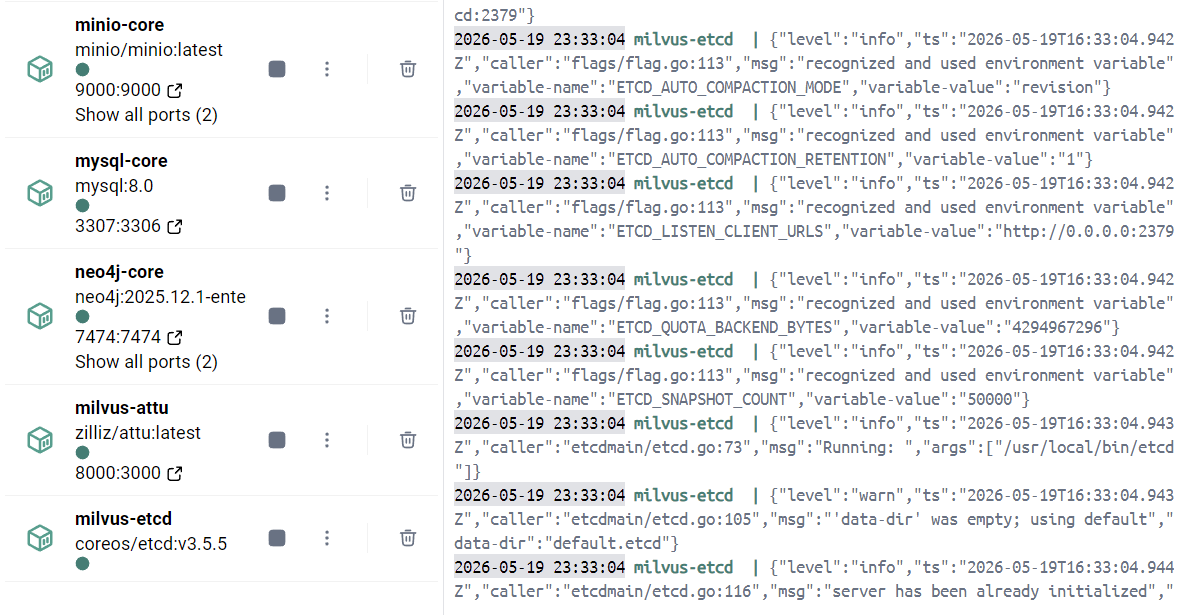
\includegraphics[width=\textwidth]{Images/ex/docker.png}
    \vspace{12pt}\caption{Docker-base infrastructure containerization and deployment}\label{fig:db_infra}
\end{figure}

Additionally, the system provides comprehensive database monitoring tools for all data containers, facilitating efficient debugging and direct tool testing.

\begin{figure}[H]
    \centering
    \begin{minipage}{0.25\textwidth}
        \centering
        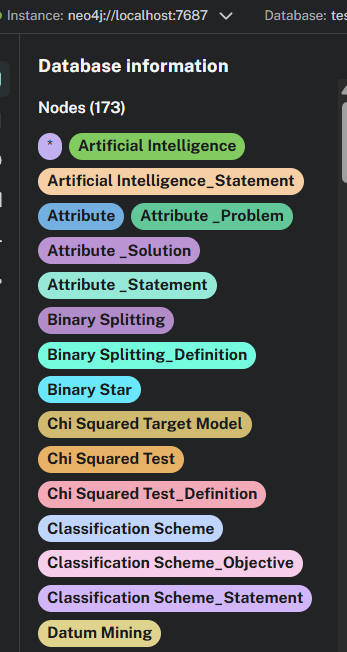
\includegraphics[width=\linewidth]{Images/ex/neo.png}
        \vspace{8pt}\caption{Neo4j Monitor Plugins}
    \end{minipage}\hfill
    \begin{minipage}{0.6\textwidth}
        \centering
        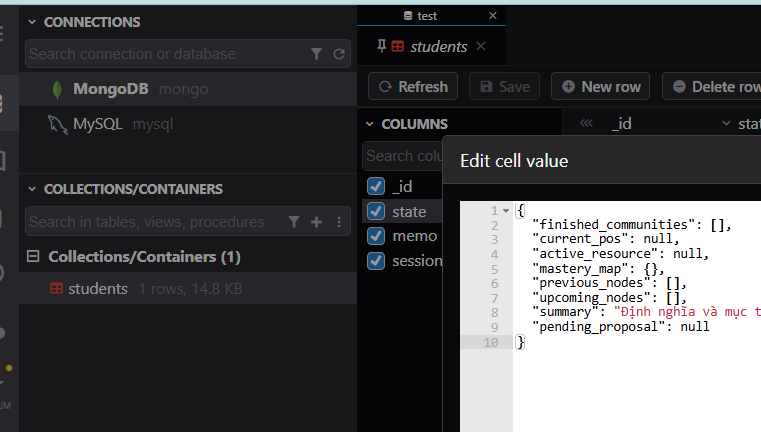
\includegraphics[width=\linewidth]{Images/ex/dbgate.png}
        \vspace{8pt}\caption{DBgate monitoring both MongoDB and SQLite}
    \end{minipage}
    \vspace{12pt}\caption{Database Admin Monitoring and Visualizing}\label{fig:db_monitor}
\end{figure}

\subsection{FastAPI App Deployment}
\begin{figure}[H]
    \centering
    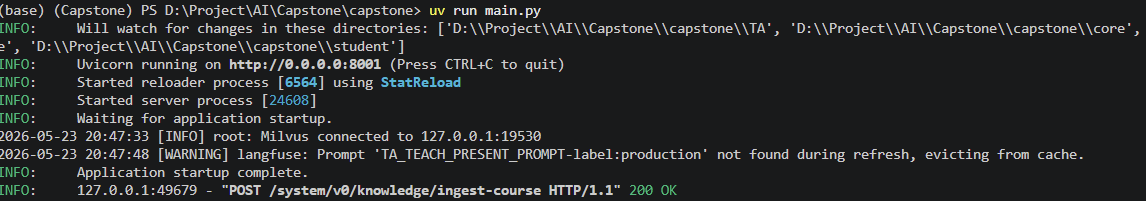
\includegraphics[width=\textwidth]{Images/ex/app_run.png}
    \vspace{12pt}\caption{FastAPI successful lifecycle start}\label{fig:app_run}
\end{figure}
The App is hosted via uvicorn. The lifespan create connection pool, initialize Singleton Modules and listen on port 8001. The Figure~\ref{fig:app_run} 
shows that all deployments are success and endpoints of main components have been publicly exposed for usage.
\section{Knowledge Module}
\subsection{Service Endpoints}
\begin{itemize}
    \item {\texttt{POST /ingest-course}}
    \begin{itemize}
        \item {Use case}: Enqueues a course ingestion request, validates the presence of uploaded PDF documents, and triggers the background processing pipeline to extract semantic concepts and construct the Knowledge Graph.
        \item {Input schema}: 
        \begin{itemize}
            \item \texttt{course\_name} (String): The title of the course being ingested.
            \item \texttt{slide\_files} (List of Strings): A list of slide file names to be processed.
            \item \texttt{textbook\_files} (List of Strings): A list of textbook file names to be processed.
            \item \texttt{reset} (Boolean): A flag indicating whether to reset the existing course data before proceeding.
        \end{itemize}
        \item {Output schema}: 
        \begin{itemize}
            \item \texttt{status} (String): The acceptance status of the background task.
            \item \texttt{message} (String): A descriptive confirmation message.
            \item \texttt{details} (Object): Additional metrics, including the count of slides and textbooks queued.
        \end{itemize}
    \end{itemize}
\end{itemize}

\subsection{Runtime}
During execution, the client transmits documents via an HTTP stream of bytes, which are subsequently loaded as PDF files. 
\begin{figure}[H]
    \centering
    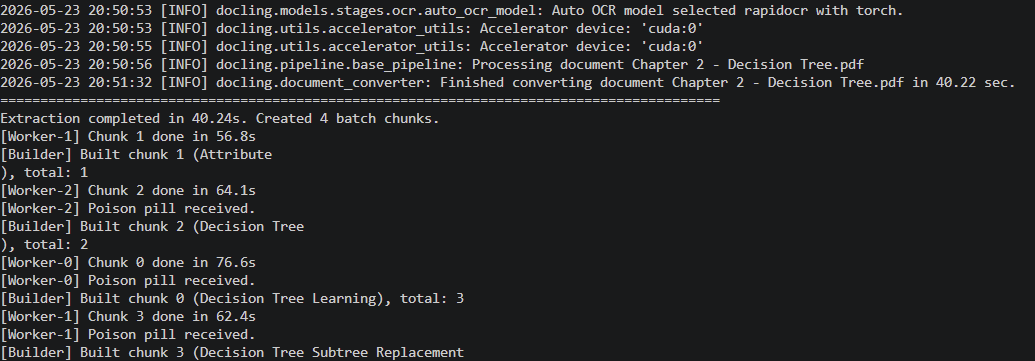
\includegraphics[width=\textwidth]{Images/ex/asynch_ingest.png}
    \vspace{12pt}\caption{Tracking Log of Asynchronous Ingestion}\label{fig:asynch_ingest}
\end{figure}
Those file goes through an asynchronous, long extraction process to formulating normalized filtered nodes and edges.

\begin{figure}[H]
    \centering
    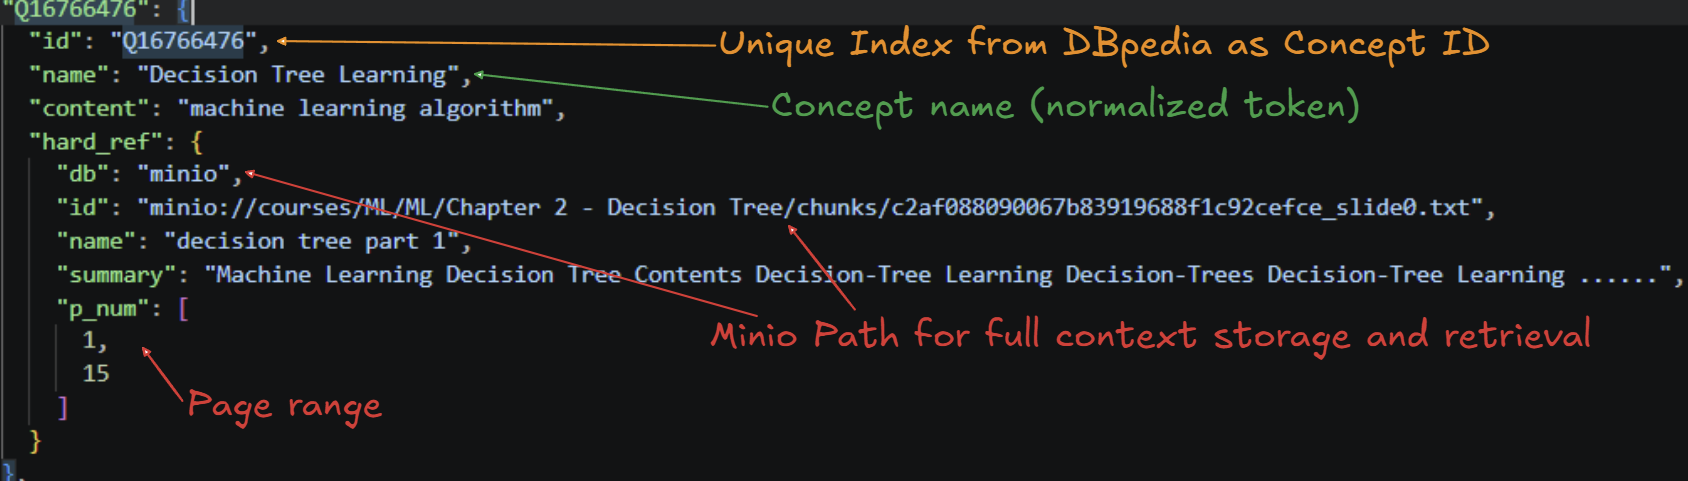
\includegraphics[width=\textwidth]{Images/ex/node.png}
    \vspace{12pt}\caption{Extracted Concept Nodes}\label{fig:node_dict}
\end{figure}
All those valuable Artifacts are pushed and saved on Neo4J. 
\begin{figure}[H]
    \centering
    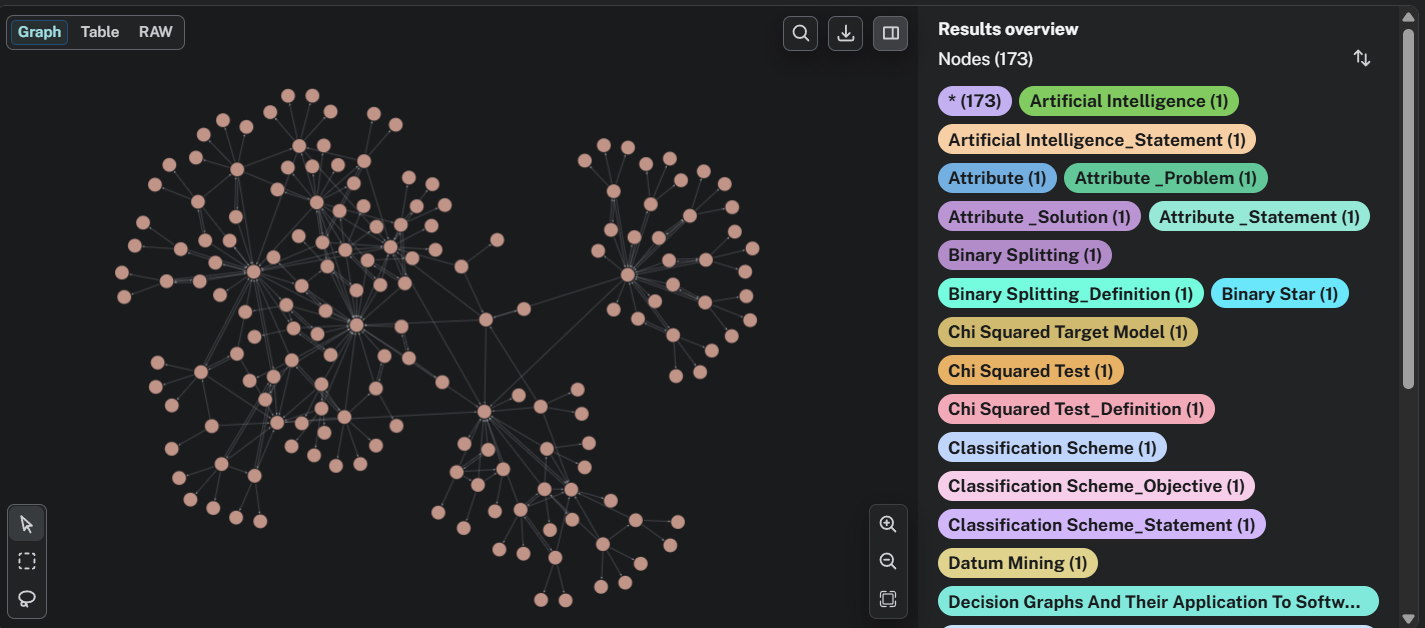
\includegraphics[width=\textwidth]{Images/ex/graph.png}
    \vspace{12pt}\caption{Completed Knowledge Graph demonstrating no concept fragmentation}\label{fig:graph_neo}
\end{figure}

However, the external knowledge base, DBpedia, occasionally provides inconsistent name and definitions. 
This manifests as words receiving inaccurate definitions or unnormalized representations.

\begin{figure}[H]
    \centering
    
\includegraphics[width=0.3\textwidth]{Images/ex/pedia_err.png}
    \vspace{12pt}\caption{DBpedia accepting unusual or unnormalized node names}\label{fig:pedia_err}
\end{figure}

Furthermore, we observed the following operational constraints:
\begin{itemize}
    \item An overly detailed Knowledge Graph becomes challenging to visualize, especially when exceeding 100 nodes and generating over 300 relationships per 20 pages.
    \item The ingestion process requires approximately 250 seconds per 50 pages, even when utilizing 3 asynchronous task workers.
\end{itemize}

\section{Student Module}
\subsection{Service Endpoints}
The Student Module exposes several key endpoints for identity and session management:

\begin{itemize}
    \item {\texttt{POST /register}}
    \begin{itemize}
        \item {Use case}: Registers new student profiles, hashes credentials, and initializes a default state document.
        \item {Input schema}:
        \begin{itemize}
            \item \texttt{student\_id} (String): The unique identifier chosen by the student.
            \item \texttt{password} (String): The plain-text password to be securely hashed.
        \end{itemize}
        \item {Output schema}:
        \begin{itemize}
            \item \texttt{detail} (String): Confirmation message of successful registration.
        \end{itemize}
    \end{itemize}

    \item {\texttt{POST /login}}
    \begin{itemize}
        \item {Use case}: Validates student credentials and generates a secure JWT authentication payload.
        \item {Input schema}:
        \begin{itemize}
            \item \texttt{username} (String): The student's unique identifier.
            \item \texttt{password} (String): The student's password.
        \end{itemize}
        \item {Output schema}:
        \begin{itemize}
            \item \texttt{access\_token} (String): The JWT payload used for subsequent authenticated requests.
            \item \texttt{token\_type} (String): The token category, typically set to "bearer".
        \end{itemize}
    \end{itemize}

    \item {\texttt{POST /session/start}}
    \begin{itemize}
        \item {Use case}: Generates a session-specific UUID token to isolate chat interactions.
        \item {Input schema}:
        \begin{itemize}
            \item \texttt{Authorization} (Header String): Bearer token (JWT) of the authenticated student.
        \end{itemize}
        \item {Output schema}:
        \begin{itemize}
            \item \texttt{session\_id} (String): A uniquely generated UUID functioning as an opaque token for a specific chat instance.
        \end{itemize}
    \end{itemize}

    \item {\texttt{DELETE /session/end}}
    \begin{itemize}
        \item {Use case}: Discards the active session token to cleanly terminate the session.
        \item {Input schema}:
        \begin{itemize}
            \item \texttt{session\_id} (Query String): The UUID of the session to terminate.
            \item \texttt{Authorization} (Header String): Bearer token (JWT) of the authenticated student.
        \end{itemize}
        \item {Output schema}: Returns HTTP 204 (No Content) indicating successful deletion.
    \end{itemize}
\end{itemize}

\subsection{Runtime}
The system demonstrates the capability to robustly handle user sessions, including detecting pre-existing users during registration or login processes.

\begin{figure}[H]
    \centering
    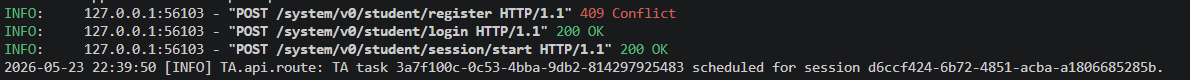
\includegraphics[width=\textwidth]{Images/ex/login.png}
    \vspace{12pt}\caption{Status 409 indicating a pre-existing student ID entry in the database. A new Session ID and access credentials are concurrently created.}\label{fig:session_login}
\end{figure}

\section{Teaching Module}
\subsection{Service Endpoints}
\begin{itemize}
    \item {\texttt{POST /chat}}
    \begin{itemize}
        \item {Use case}: Serves as the primary tutoring interface. It receives user queries alongside their active session IDs, subsequently executing the multi-agent LangGraph tutoring pipelines to formulate contextual responses.
        \item {Input schema}:
        \begin{itemize}
            \item \texttt{session\_id} (String): The UUID for the active chat session authenticated by the user.
            \item \texttt{user\_input} (String): The actual query or message submitted by the student.
            \item \texttt{language} (String): The language preference toggle (e.g., "vn" or "eng").
        \end{itemize}
        \item {Output schema}:
        \begin{itemize}
            \item \texttt{task\_id} (String): A unique identifier assigned to track the asynchronous background task.
            \item \texttt{status} (String): The initial state, typically indicating receipt of the request.
            \item \texttt{agent} (String): The default agent assigned to process the workflow.
        \end{itemize}
    \end{itemize}

    \item {\texttt{GET /chat/status/\{task\_id\}}}
    \begin{itemize}
        \item {Use case}: Sends system status back to the client while waiting. The streaming output can be included here as well.
        \item {Input schema}:
        \begin{itemize}
            \item \texttt{task\_id} (Path String): The unique identifier of the background task being polled.
        \end{itemize}
        \item {Output schema}:
        \begin{itemize}
            \item \texttt{status} (String): The current operational state (e.g., "working", "finished", or "Fail").
            \item \texttt{agent\_name}, \texttt{intent}, \texttt{thought} (String, optional): Metadata illustrating the agent's current step, intended action, and reasoning.
            \item \texttt{result} (Object, optional): Available upon completion, containing the final \texttt{message} string and optional \texttt{ui\_action} dictionaries.
            \item \texttt{error} (String, optional): Descriptive failure logs in the event of pipeline exceptions.
        \end{itemize}
    \end{itemize}
\end{itemize}
\subsection{Runtime}
Upon submitting a query, the client interface consistently monitors the agentic progress, displaying the current status and the active agent. Once the pipeline concludes, the service transmits the final text result back to the client.

\begin{figure}[H]
    \centering
    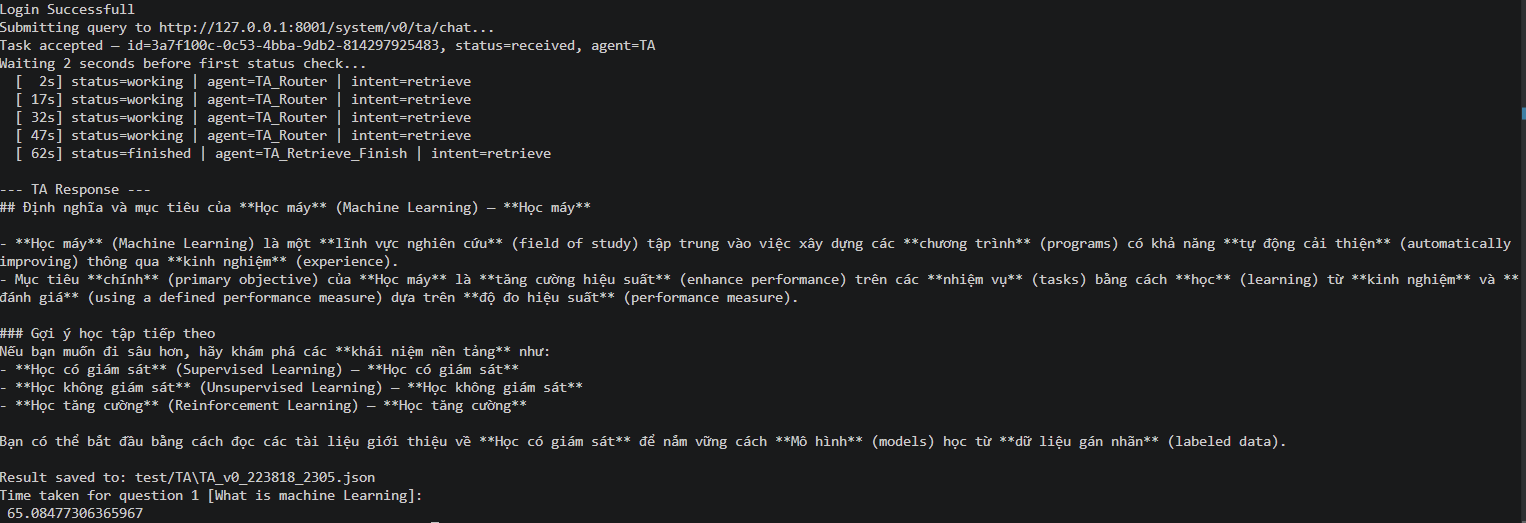
\includegraphics[width=\textwidth]{Images/ex/full_TA_output_1.png}
    \vspace{12pt}\caption{Client-side interface displaying the agentic interaction flow}\label{fig:client_answer}
\end{figure}

Simultaneously, the system persistently logs and saves the outcomes of agentic tool executions and messages, facilitating potential reusability and analytical reviews.

\begin{figure}[H]
    \centering
    \begin{minipage}{0.48\textwidth}
        \centering
        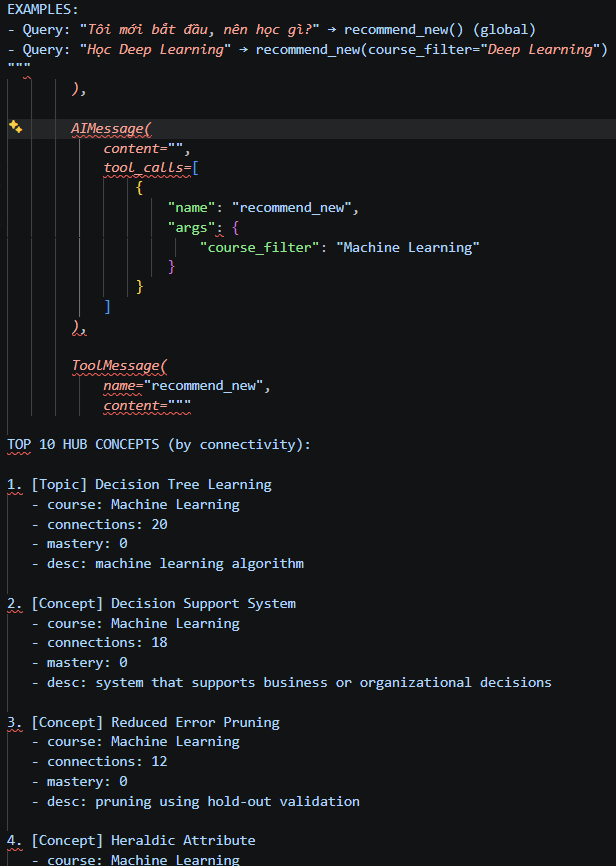
\includegraphics[width=\linewidth]{Images/ex/tool_mess.png}
    \end{minipage}\hfill
    \begin{minipage}{0.48\textwidth}
        \centering
        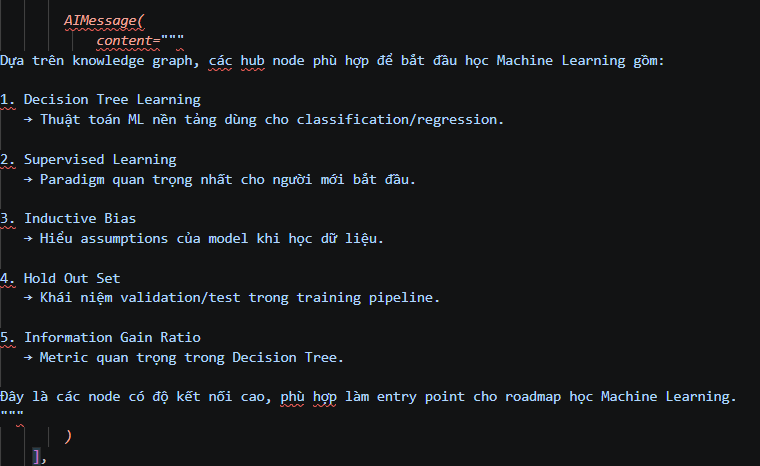
\includegraphics[width=\linewidth]{Images/ex/ai_mess.png}
    \end{minipage}
    \vspace{12pt}\caption{2 snippet of Logged Agent Workflow result}\label{fig:workflow_log}
\end{figure}

Currently, the core teaching workflow remains under active development, while the retrieval and roadmap workflows have
 demonstrated promising initial results. Moving forward, comprehensive benchmarks and advanced evaluation metrics will 
 be investigated to formally assess the system's efficiency in automated, intelligent education expertise.